\newif\ifshowsolutions
\showsolutionstrue
\input{../preamble}



%%%%%%%%%%%%%%%%%%%%%%%%%%%%%%
% HEADER
%%%%%%%%%%%%%%%%%%%%%%%%%%%%%%

\chead{
  {\vbox{
      \vspace{2mm}
      \large
      Machine Learning \& Data Mining \hfill
      Caltech CS/CNS/EE 155 \hfill \\[1pt]
      Set 5\hfill
      February 2019\\
    }
  }
}

\begin{document}
\pagestyle{fancy}



\section{SVD and PCA [35 Points]}

\problem[3] 

\begin{solution}
\end{solution}

\newpage
\problem[4] 

\begin{solution}
 
\end{solution}

\newpage
\problem[5] 

\begin{solution}

\end{solution}

\newpage
\problem[3] 

\begin{solution}

\end{solution}


\newpage
\problem[3] .

\begin{solution}

\end{solution}

\newpage
\problem[3] 

\begin{solution}

\end{solution} 

\newpage
\problem[4] 

\begin{solution}

\end{solution}


\newpage
\problem[4] 

\begin{solution}

\end{solution}

\newpage
\problem[4] 
\begin{solution}
\end{solution}

\newpage
\problem[2] 
\begin{solution}

\end{solution}


\newpage
\section{Matrix Factorization [30 Points]}

\problem[5]

\begin{solution}

\end{solution}

\newpage
\problem[5]

\begin{solution}

\end{solution}

\newpage
\problem[10]

\begin{solution}
See 2D.py and prob2utils.py for the solution code.
\end{solution}

\newpage
\problem[5]

\begin{solution}

%
%\begin{figure}[H]
%\begin{center}
%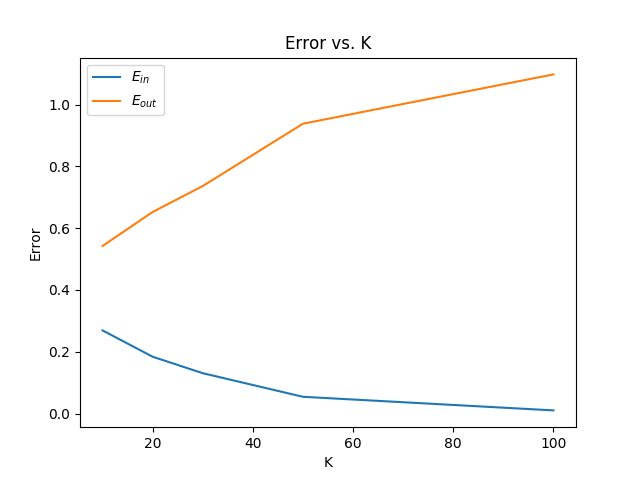
\includegraphics[width=0.8\textwidth]{plots/2d.png}
%\caption{Unregularized factorization}
%\label{fig:UnregFact}
%\end{center}
%\end{figure}


\end{solution}

\newpage
\problem[5]

\begin{solution}


%\begin{figure}[H]
%\begin{center}
%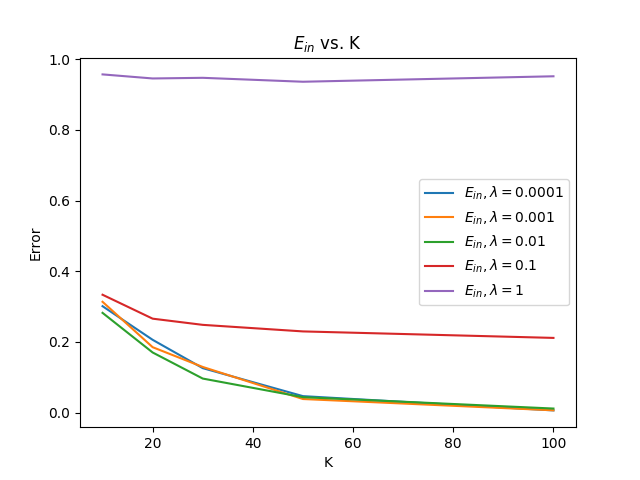
\includegraphics[width=0.45\textwidth]{plots/2e_ein.png}
%\caption{$E_{in}$ vs $k$ for different $\lambda$}
%\label{fig:RegFact1}
%\end{center}
%\end{figure}

%\begin{figure}[H]
%\begin{center}
%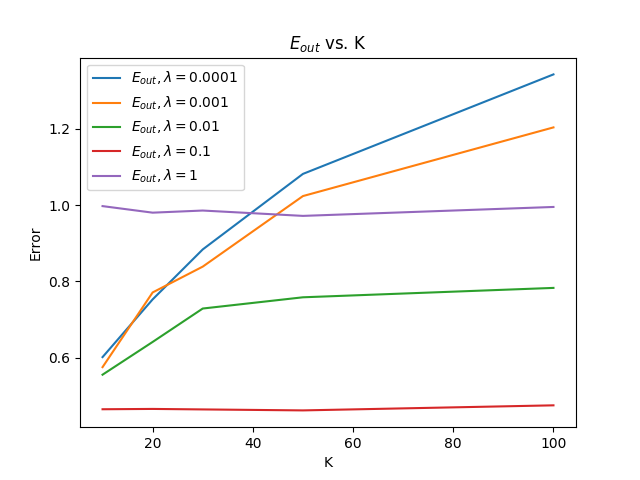
\includegraphics[width=0.45\textwidth]{plots/2e_eout.png}
%\caption{$E_{out}$ vs $k$ for different $\lambda$}
%\label{fig:RegFact2}
%\end{center}
%\end{figure}

 
\end{solution}






\newpage
\section{Word2Vec Principles [35 Points]}

\problem[5]


\begin{solution}

\end{solution}


\newpage
\problem[10]

\begin{solution}

\end{solution}


\newpage
\problem[3]


\begin{solution}

\end{solution}




\newpage
\problem[10]



\begin{solution}
See solution code in P3C.py
\end{solution}


\newpage
\problem[2]


\begin{solution}

\end{solution}

\newpage
\problem[2]

\begin{solution}

\end{solution}

\newpage
\problem[1]

\begin{solution}

%\begin{verbatim}
%
%\end{verbatim}

\end{solution}
\newpage

\problem[2]

\begin{solution}


\end{solution}

\end{document}

